\documentclass[11pt]{report}

% USE WITH \newgeometry
\usepackage[paper=a4paper, top=1in, bottom=1in, left=1.25in, right=1.25in]{geometry}
\usepackage[font=scriptsize]{caption}
\usepackage[utf8]{inputenc}
\usepackage[italian]{babel}
\usepackage{listings}
\usepackage{hyperref}
\usepackage{graphicx}
\usepackage{subcaption}
\usepackage{enumitem}
\usepackage{float}
\usepackage{color}
\usepackage[export]{adjustbox}
% \usepackage[font=small,labelfont=bf]{caption}


%% SETTINGS %%

% Image base path
\graphicspath{{img/}}

% Custom colors
\definecolor{deepblue}{rgb}{0,0,0.5}
\definecolor{deepred}{rgb}{0.6,0,0}
\definecolor{deepgreen}{rgb}{0,0.5,0}

% Default fixed font does not support bold face
\DeclareFixedFont{\ttb}{T1}{txtt}{bx}{n}{8} % for bold
\DeclareFixedFont{\ttm}{T1}{txtt}{m}{n}{8}  % for normal

% Necessary for italian documents
\frenchspacing

% Line height
\linespread{1.3}
% Table of content deep
\setcounter{tocdepth}{3}
\setcounter{secnumdepth}{4}

% Link configuration
\hypersetup{
    pdfpagemode={UseOutlines},
    bookmarksopen,
    pdfstartview={FitH},
    colorlinks,
    linkcolor={black},
    citecolor={black},
    urlcolor={black}
}

% pdf infos
\pdfinfo{
    /Title    Thesis
    /Author   Your name
    /Subject  Triennial Thesis
    /Keywords Thesis, University, Triennial Thesis, DISIM, L'Aquila
}

% CUSTOM COMMANDS

% Python code style
\newcommand\pythonstyle{\lstset{
    language=Python,
    basicstyle=\ttm,
    otherkeywords={self, def},
    keywordstyle=\ttb\color{deepblue},
    emph={MyClass,__init__},
    emphstyle=\ttb\color{deepred},
    commentstyle=\color{deepgreen},
    stringstyle=\color{deepgreen},
    frame=lines,
    breaklines=true,
    breakatwhitespace=true,
    showstringspaces=false,
    numbers=left,
    numberstyle=\footnotesize,
}}

% Python for inline
\newcommand\pythoninline[1]{{\pythonstyle\lstinline!#1!}}

% Python for external files
\newcommand\pythonexternal[2][]{{
    \vspace{0.5cm}
    \pythonstyle
    \lstinputlisting[#1]{#2}
    \vspace{0.5cm}
}}


% Java code style
\newcommand\javastyle{\lstset{
    language=Java,
    basicstyle=\ttm,
    otherkeywords={self, def},
    keywordstyle=\ttb\color{deepblue},
    emph={Class},
    emphstyle=\ttb\color{deepred},
    commentstyle=\color{deepgreen},
    stringstyle=\color{deepgreen},
    frame=lines,
    breaklines=true,
    breakatwhitespace=true,
    showstringspaces=false,
    numbers=left,
    numberstyle=\footnotesize,
}}  

% Java for inline
\newcommand\javainline[1]{{\javastyle\lstinline!#1!}}

% Java for external files
\newcommand\javaexternal[2][]{{
    \vspace{0.5cm}
    \javastyle
    \lstinputlisting[#1]{#2}
    \vspace{0.5cm}
}}

% Create a custom paragraph with newline at the end
\newcommand{\myparagraph}[1]{\paragraph*{\normalfont#1}\mbox{}\\}


%% BEGIN DOCUMENT %%

\begin{document}

    % Frontispiece
    % FRONTISPIECE

\begin{figure}[h]
    \begin{minipage}[t]{0.2\textwidth}
        
\includegraphics[width=\textwidth]{./img/univaq_logo.png}
    \end{minipage}
    \hfill
    \begin{minipage}[t]{0.15\textwidth}
        % Inserisci il logo del tuo dipartimento nella cartella img e importalo qui
        
\includegraphics[width=\textwidth]{./img/disim_logo_descr.png}
    \end{minipage}
\end{figure}

\vspace{1.5cm}

% University and department
\begin{center}
    {\LARGE Università degli Studi dell'Aquila}
    % Cambiare anche il logo in alto a destra del frontespizio
    \myparagraph{Inserisci il nome del tuo dipartimento per esteso}
    \myparagraph{Inserisci il nome del tuo corso di laurea per esteso}
    \vspace{.7cm}
    \myparagraph{\textbf{Tesi di Laurea}}
    \vspace{2cm}
    \large{{\textbf{\emph{
                Questo è il fantastico titolo della mia tesi di laurea triennale con testo
                volutamente lungo
            }}}
    }
    
    \vspace{3.5cm}

    % Tab
    \begin{tabular}{c}
        \normalsize\textbf{Relatore}\\\\
        \normalsize{Prof. Pinco Pallino}
    \end{tabular}
    \hfill
    \begin{tabular}{c}
        \normalsize\textbf{Laureando}\\\\
        \normalsize{Mario Rossi}
    \end{tabular}

    \vspace{4.5cm}

    % Settare l'anno accademico in cui ci sta laureando
    \rule{10cm}{.1mm}\\ {\large Anno Accademico 2017-2018}

\end{center}
    %\clearpage\null\newpage
    
\begin{flushright}
    \emph{Al mio caro carissimo, \\grazie per avermi fatto laureare.}
\end{flushright}

    %\clearpage\null\newpage
    % Index
    \tableofcontents
    %\newpage
    % Left alignment
    \begin{flushleft}
        % Chapters
        \chapter*{Introduzione}\label{Introduzione}

Lorem ipsum dolor sit amet, consectetur adipisci elit, sed eiusmod tempor incidunt ut labore et dolore magna aliqua. Ut enim ad minim veniam, quis nostrum exercitationem ullam corporis suscipit laboriosam, nisi ut aliquid ex ea commodi consequatur. Quis aute iure reprehenderit in voluptate velit esse cillum dolore eu fugiat nulla pariatur. Excepteur sint obcaecat cupiditat non proident, sunt in culpa qui officia deserunt mollit anim id est laborum.\\
Lorem ipsum dolor sit amet, consectetur adipisci elit, sed eiusmod tempor incidunt ut labore et dolore magna aliqua. Ut enim ad minim veniam, quis nostrum exercitationem ullam corporis suscipit laboriosam, nisi ut aliquid ex ea commodi consequatur. Quis aute iure reprehenderit in voluptate velit esse cillum dolore eu fugiat nulla pariatur. Excepteur sint obcaecat cupiditat non proident, sunt in culpa qui officia deserunt mollit anim id est laborum.\\
Lorem ipsum dolor sit amet, consectetur adipisci elit, sed eiusmod tempor incidunt ut labore et dolore magna aliqua. Ut enim ad minim veniam, quis nostrum exercitationem ullam corporis suscipit laboriosam, nisi ut aliquid ex ea commodi consequatur. Quis aute iure reprehenderit in voluptate velit esse cillum dolore eu fugiat nulla pariatur. Excepteur sint obcaecat cupiditat non proident, sunt in culpa qui officia deserunt mollit anim id est laborum.\\
Lorem ipsum dolor sit amet, consectetur adipisci elit, sed eiusmod tempor incidunt ut labore et dolore magna aliqua. Ut enim ad minim veniam, quis nostrum exercitationem ullam corporis suscipit laboriosam, nisi ut aliquid ex ea commodi consequatur. Quis aute iure reprehenderit in voluptate velit esse cillum dolore eu fugiat nulla pariatur. Excepteur sint obcaecat cupiditat non proident, sunt in culpa qui officia deserunt mollit anim id est laborum.\\
Lorem ipsum dolor sit amet, consectetur adipisci elit, sed eiusmod tempor incidunt ut labore et dolore magna aliqua. Ut enim ad minim veniam, quis nostrum exercitationem ullam corporis suscipit laboriosam, nisi ut aliquid ex ea commodi consequatur. Quis aute iure reprehenderit in voluptate velit esse cillum dolore eu fugiat nulla pariatur. Excepteur sint obcaecat cupiditat non proident, sunt in culpa qui officia deserunt mollit anim id est laborum.

        \chapter{Capitolo 1}\label{Capitolo1}
Lorem ipsum dolor sit amet, consectetur adipisci elit, sed eiusmod tempor incidunt ut labore et dolore magna aliqua. Ut enim ad minim veniam, quis nostrum exercitationem ullam corporis suscipit laboriosam, nisi ut aliquid ex ea commodi consequatur. Quis aute iure reprehenderit in voluptate velit esse cillum dolore eu fugiat nulla pariatur. Excepteur sint obcaecat cupiditat non proident, sunt in culpa qui officia deserunt mollit anim id est laborum.\\

Esempio di inserimento immagini:

\vspace{0.5cm}
\begin{figure}[H]
    \centering
    \begin{subfigure}[b]{0.4\linewidth}
        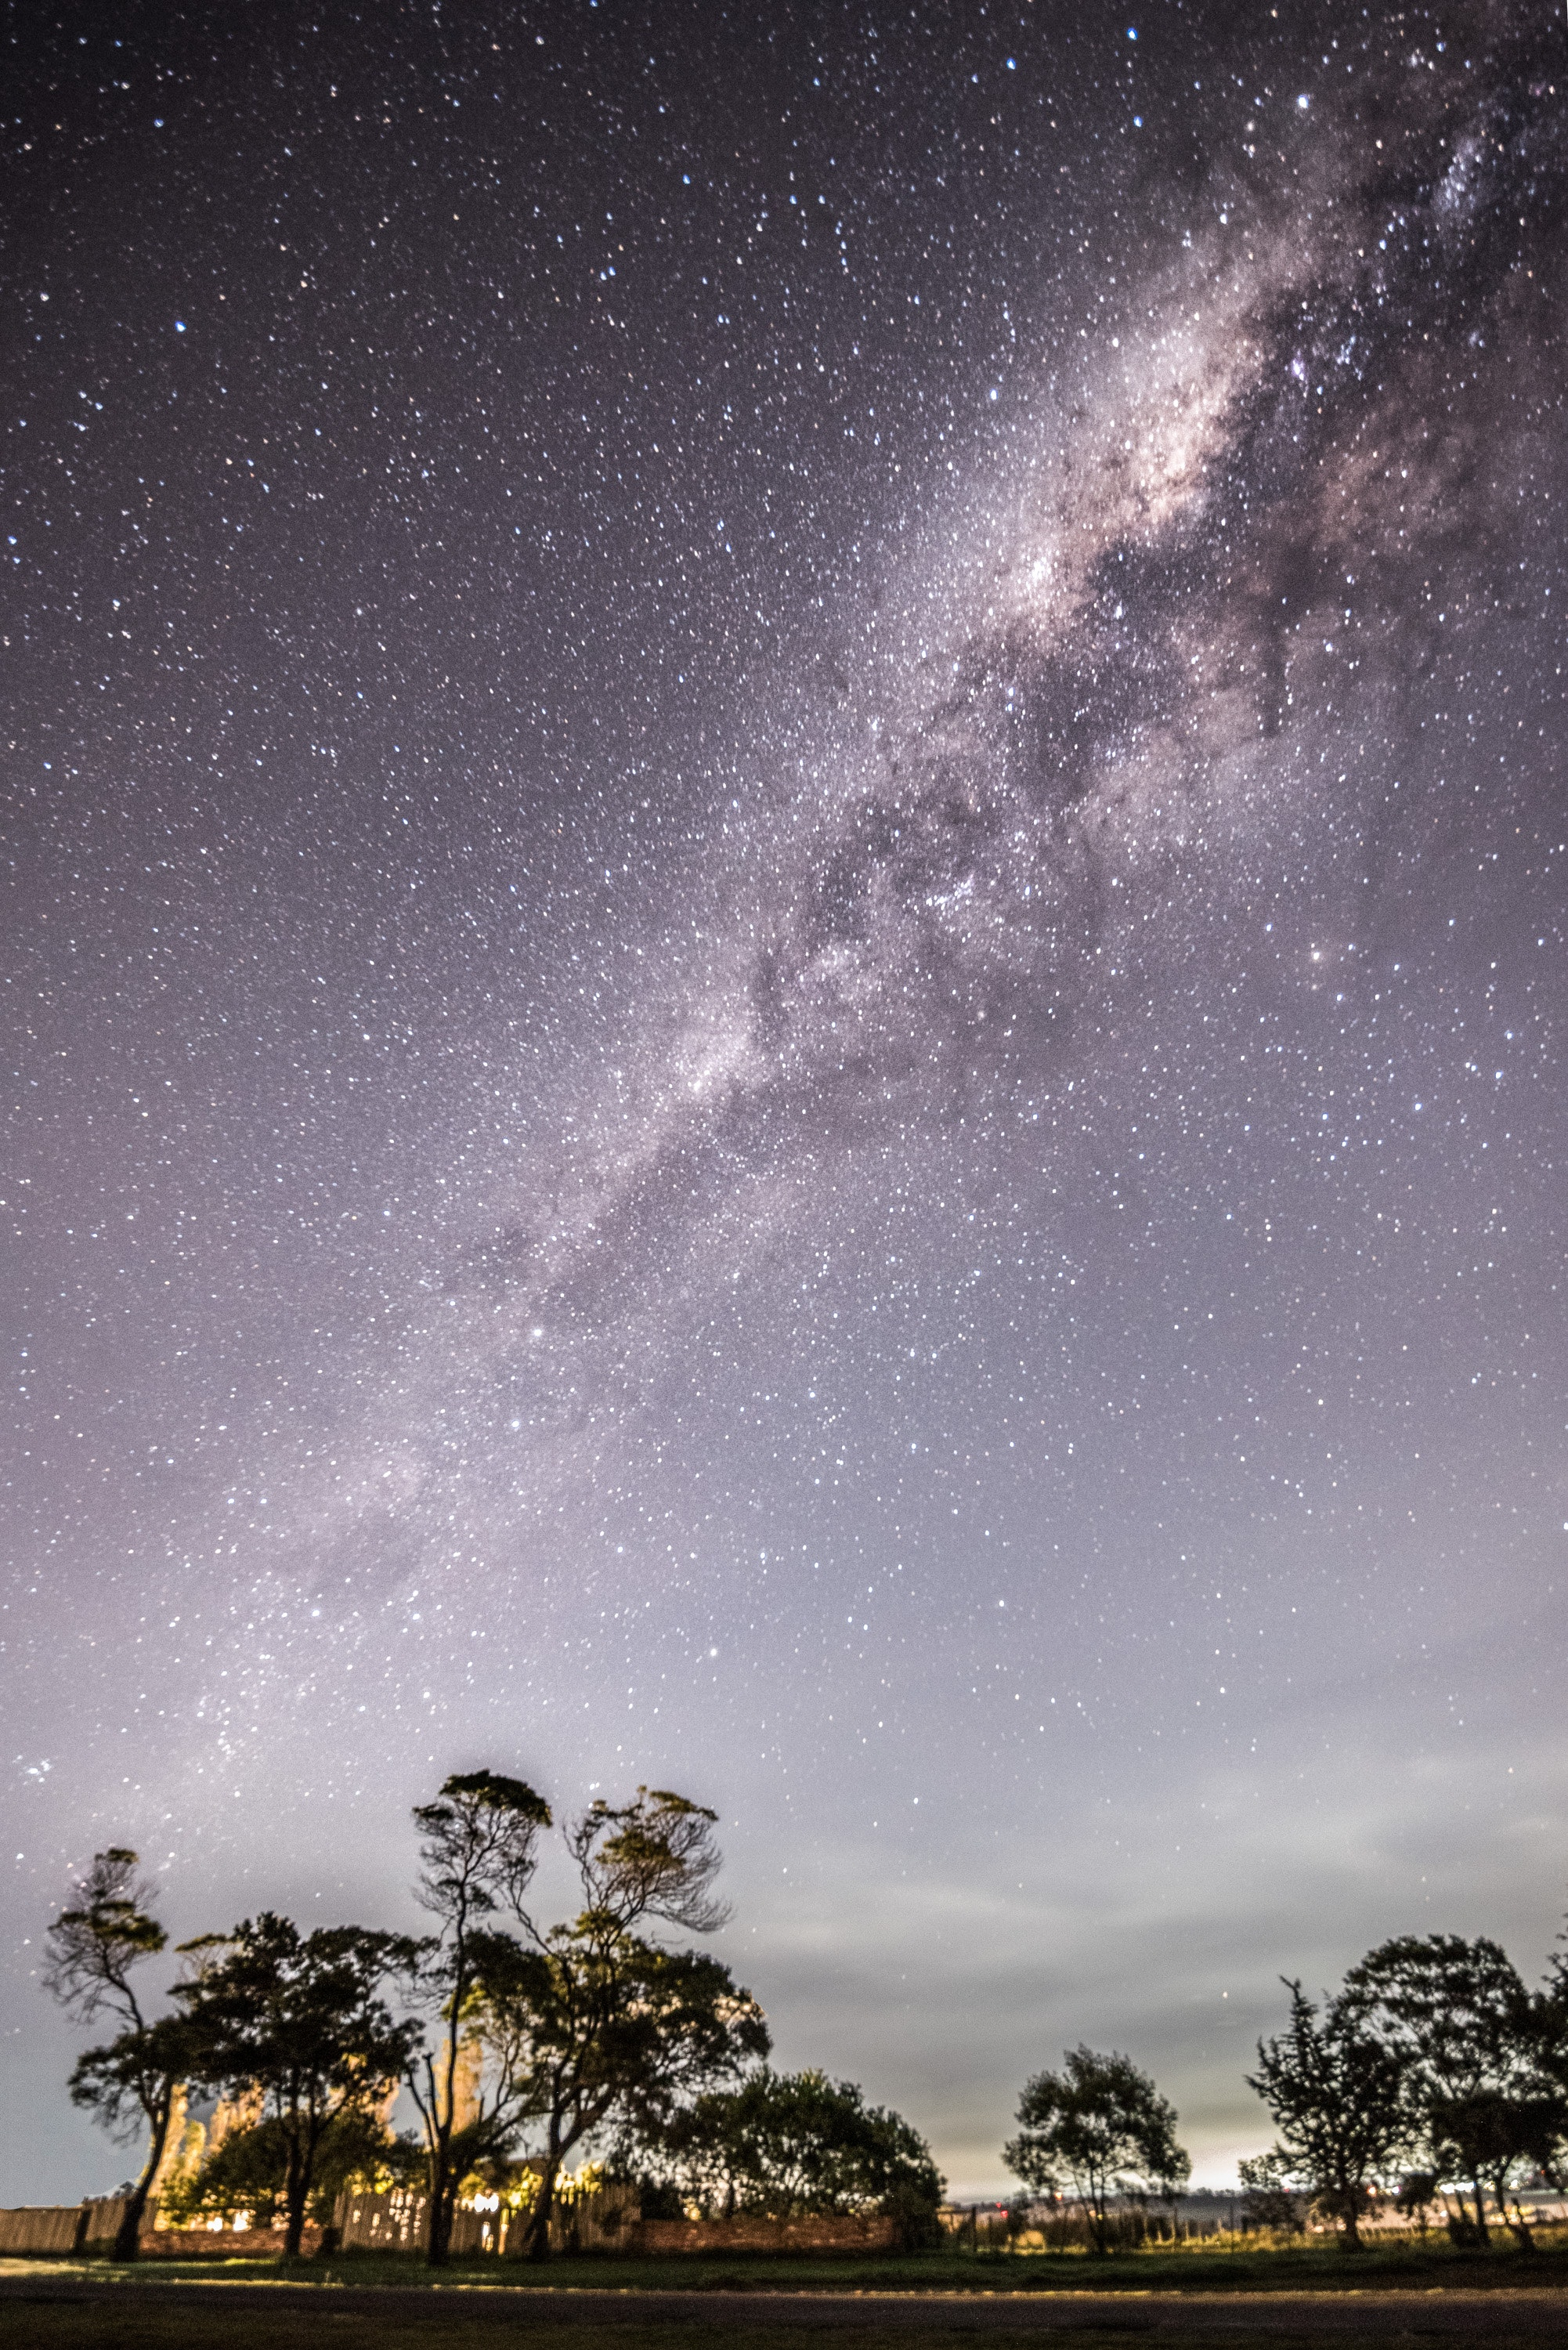
\includegraphics[width=\linewidth]{./image1.jpg}
        \caption{Immagine 1.}
    \end{subfigure}
    \hspace{1.3cm}
    \begin{subfigure}[b]{0.4\linewidth}
        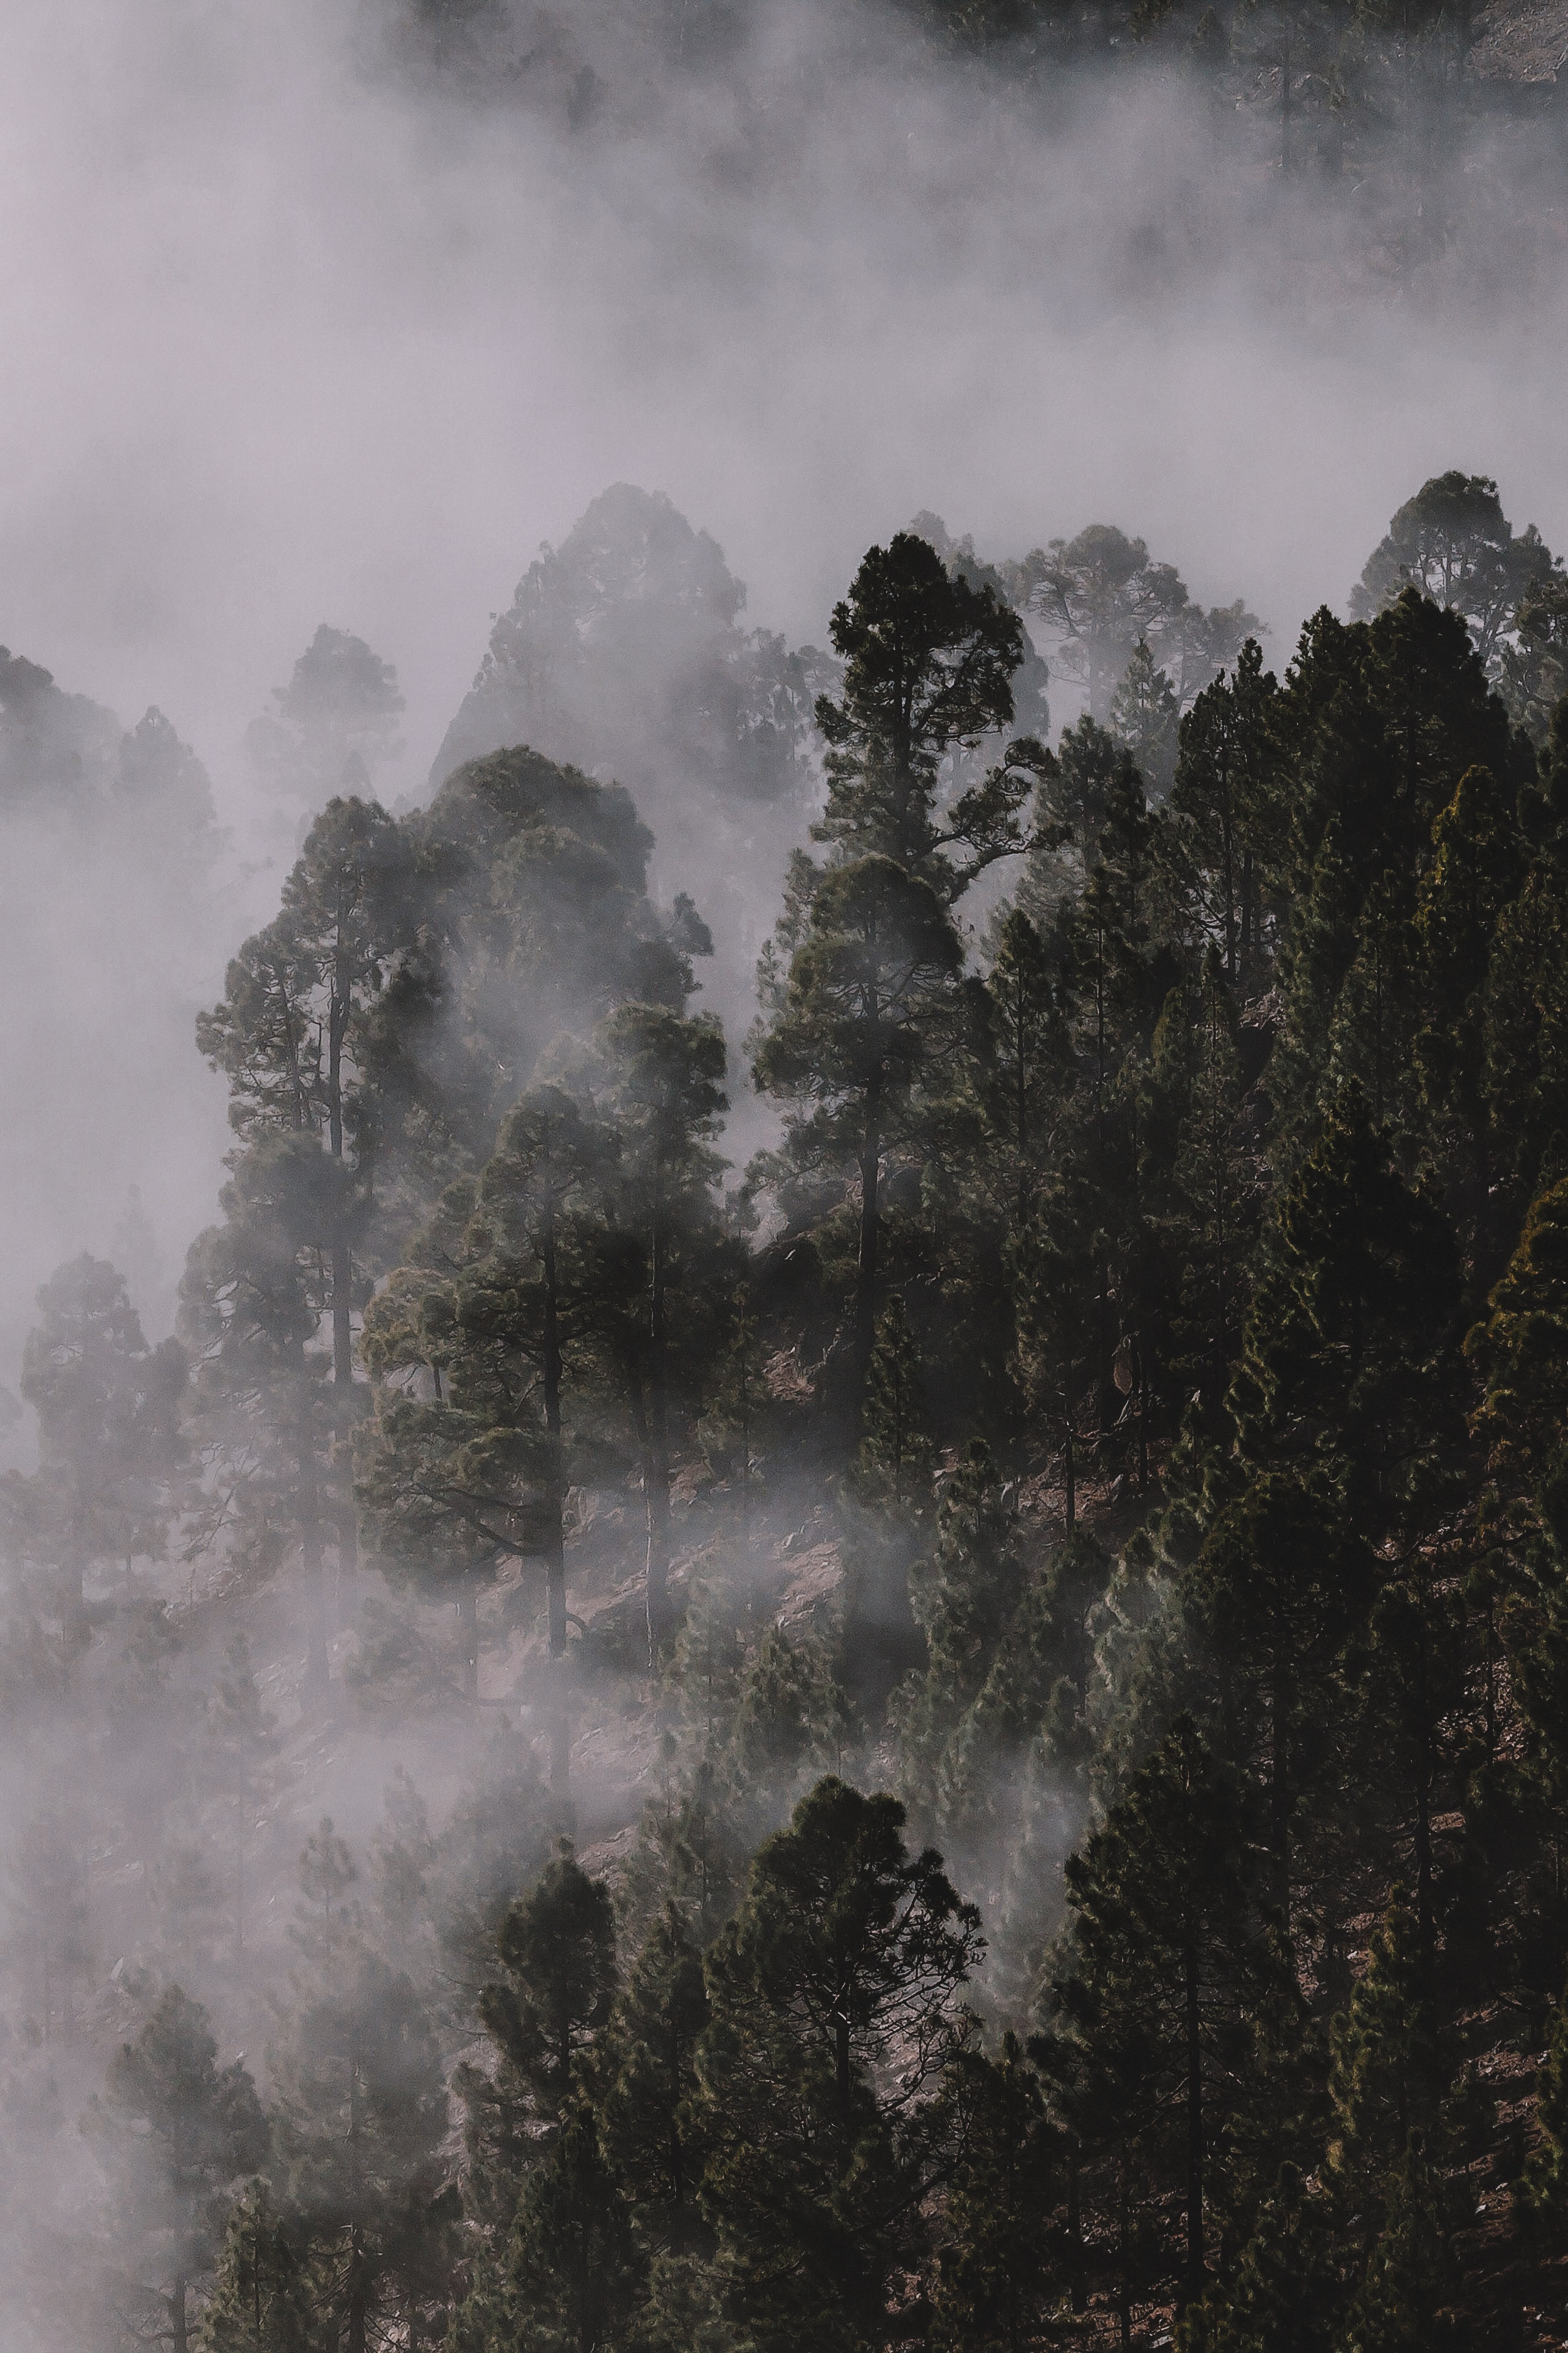
\includegraphics[width=\linewidth]{./image2.jpg}
        \caption{Immagine 2.}
    \end{subfigure}
    \vspace{.5cm}
    \caption{Breve descrizione delle immagini}
\end{figure}
\vspace{0.5cm}

\newpage

% INIZIO SEZIONE
\section{Paragrafo 1}\label{Paragrafo1}
Lorem ipsum dolor sit amet, consectetur adipisci elit, sed eiusmod tempor incidunt ut labore et dolore magna aliqua.

% INIZIO SEZIONE
\section{Paragrafo 2}\label{Paragrafo2}
Lorem ipsum dolor sit amet, consectetur adipisci elit, sed eiusmod tempor incidunt ut labore et dolore magna aliqua.

% INIZIO SOTTOSEZIONE
\subsection{Sottoparagrafo 1}\label{Sottoparagrafo 1}
Lorem ipsum dolor sit amet, consectetur adipisci elit, sed eiusmod tempor incidunt ut labore et dolore magna aliqua.

% INIZIO SOTTOSEZIONE
\subsection{Sottoparagrafo 2}\label{Sottoparagrafo 2}

Esempio di lista:

\begin{itemize}[noitemsep]
    \item Primo elemento della lista
    \item Secondo elemento della lista
    \item Terzo elemento della lista
\end{itemize}


% INIZIO SOTTOSEZIONE
\subsection{Sottoparagrafo 3}\label{Sottoparagrafo 3}
Esempi di riferimento alla bibliografia:

Come riportato in \cite{6223430}.\\
Come riportato in \cite{adamgeitgey}.\\
Come riportato in \cite{Kazemi_2014_CVPR}.\\
Come riportato in \cite{Schroff_2015_CVPR}.\\
Come riportato in \cite{SourceAFIS}.

        \chapter{Capitolo 2}\label{Capitolo 2}

% INIZIO SEZIONE
\section{Paragrafo 3}\label{Paragrafo3}

% INIZIO SOTTOSEZIONE
\subsection{Sottoparagrafo 4}\label{Sottoparagrafo4}

% INIZIO SOTTOSOTTOSEZIONE
\subsubsection{Sottosottoparagrafo 1}\label{Sottosottoparagrafo1}

Esempio di codice Python inline: \pythoninline{print('Hello World')}

Esempio importazione di un blocco di codice Python:

\pythonexternal{code/hello_world.py}

Esempio di codice Java inline: \javainline{System.out.println("Hello World");}

Esempio importazione di un blocco di codice Java:

\javaexternal{code/HelloWorld.java}

% INIZIO SOTTOSOTTOSEZIONE
\subsubsection{Sottoparagrafo 5}\label{Sottoparagrafo5}

Esempio di tabella:

\begin{table}[H]
    \centering
    \begin{tabular}{|c|c|c|c|c|}
    \hline
    \textbf{Colonna 1}  & \textbf{Colonna 2}    & \textbf{Colonna 3}     & \textbf{Colonna 4}      \\ \hline
    0.49                & 112                   & 86                     & 26                      \\ \hline
    0.43                & 112                   & 106                    & 6                       \\ \hline
    0.42                & 112                   & 111                    & 1                       \\ \hline
    0.41                & 112                   & 111                    & 1                       \\ \hline
    \end{tabular}
    \caption{Descrizione tabella.}
\end{table}


        \chapter{Conclusioni}\label{Conclusioni}
Lorem ipsum dolor sit amet, consectetur adipisci elit, sed eiusmod tempor incidunt ut labore et dolore magna aliqua. Ut enim ad minim veniam, quis nostrum exercitationem ullam corporis suscipit laboriosam, nisi ut aliquid ex ea commodi consequatur. Quis aute iure reprehenderit in voluptate velit esse cillum dolore eu fugiat nulla pariatur. Excepteur sint obcaecat cupiditat non proident, sunt in culpa qui officia deserunt mollit anim id est laborum.\\
Lorem ipsum dolor sit amet, consectetur adipisci elit, sed eiusmod tempor incidunt ut labore et dolore magna aliqua. Ut enim ad minim veniam, quis nostrum exercitationem ullam corporis suscipit laboriosam, nisi ut aliquid ex ea commodi consequatur. Quis aute iure reprehenderit in voluptate velit esse cillum dolore eu fugiat nulla pariatur. Excepteur sint obcaecat cupiditat non proident, sunt in culpa qui officia deserunt mollit anim id est laborum.\\
Lorem ipsum dolor sit amet, consectetur adipisci elit, sed eiusmod tempor incidunt ut labore et dolore magna aliqua. Ut enim ad minim veniam, quis nostrum exercitationem ullam corporis suscipit laboriosam, nisi ut aliquid ex ea commodi consequatur. Quis aute iure reprehenderit in voluptate velit esse cillum dolore eu fugiat nulla pariatur. Excepteur sint obcaecat cupiditat non proident, sunt in culpa qui officia deserunt mollit anim id est laborum.
        \chapter*{Ringraziamenti}
Giunto al termine di questo percorso accademico è doveroso ringraziare tutti coloro che mi hanno affiancato durante il tragitto.

\vspace{.4cm}

Lorem ipsum dolor sit amet, consectetur adipisci elit, sed eiusmod tempor incidunt ut labore et dolore magna aliqua. Ut enim ad minim veniam, quis nostrum exercitationem ullam corporis suscipit laboriosam, nisi ut aliquid ex ea commodi consequatur. Quis aute iure reprehenderit in voluptate velit esse cillum dolore eu fugiat nulla pariatur. Excepteur sint obcaecat cupiditat non proident, sunt in culpa qui officia deserunt mollit anim id est laborum.
\vspace{.4cm}

Lorem ipsum dolor sit amet, consectetur adipisci elit, sed eiusmod tempor incidunt ut labore et dolore magna aliqua. Ut enim ad minim veniam, quis nostrum exercitationem ullam corporis suscipit laboriosam, nisi ut aliquid ex ea commodi consequatur.

\vspace{.4cm}

Lorem ipsum dolor sit amet, consectetur adipisci elit, sed eiusmod tempor incidunt ut labore et dolore magna aliqua. Ut enim ad minim veniam, quis nostrum exercitationem ullam corporis suscipit laboriosam, nisi ut aliquid ex ea commodi consequatur. Quis aute iure reprehenderit in voluptate velit esse cillum dolore eu fugiat nulla pariatur.

\vspace{.4cm}

Lorem ipsum dolor sit amet, consectetur adipisci elit, sed eiusmod tempor incidunt ut labore et dolore magna aliqua.

\vspace{.4cm}

Lorem ipsum dolor sit amet, consectetur adipisci elit, sed eiusmod tempor incidunt ut labore et dolore magna aliqua.
    \end{flushleft}
    % References
    \bibliographystyle{plain}
    \bibliography{references.bib}

\end{document}
